% Generate boilerplate to create a document with a title page, name, date with a report style
% Usage: \report{Title}{Name}{Date}

\documentclass{report}

\usepackage{graphicx}  % For including images
\usepackage{amsmath}   % For mathematical symbols and environments
\usepackage{hyperref}  % For hyperlinks
\usepackage{wrapfig}  % For wrapping text around figures

% Command to create the title page
\newcommand{\report}[3]{
    \title{#1}
    \author{#2}
    \date{#3}
    \maketitle
}

\begin{document}

% Create the title page
\report{Lyapunov Orbits}{Your Name}{\today}


\newpage

\section*{Lyapunov Orbits}
Lyapunov orbits are planar symmetric periodic orbits around the collinear points for the 3CRBP.
In order to find such solutions, the Jacobian of the linearized dynamical model around the 
equilibrium point is considered, and through diagonalization, 
two real eigenvalues (one positive $\boldsymbol{E_u}$ and one negative $\boldsymbol{E_s}$) 
and one complex pair $\boldsymbol{E_{c1}}$, $\boldsymbol{E_{c2}}$ is found.\\\\
Periodic motion is possible only in the subspace spanned by the eigenvectors corresponding to the complex eigenvalues.
Deriving the linearized equation of motion in this subspace, the state equation for a Lyapunov orbit is obtained as:
\begin{equation}
    \boldsymbol{x} = \boldsymbol{x_L} + \alpha_0(\cos(\omega t)Re({\boldsymbol{E_{c1}}}) - \sin(\omega t)Im({\boldsymbol{E_{c1}}})
\end{equation}
with $\alpha_0$ the amplitude of the periodic motion, $\omega$ the frequency of the motion, and $\boldsymbol{x_L}$ the equilibrium point.
The linearization will eventually diverge, and the periodic motion will be accurate only for small amplitudes. \\\\
To improve the accuracy of the solution and make possible the computation of a family of periodic orbits, the problem is formulated as a two-point boundary value problem (TPBVP), thanks to the simmetries of the 3CRBP.
A shooting method is then employed to solve the TPBVP, and a first nonlinear Lyapunov orbit is found from the linear guess.\\\\
Once a first solution is found, a continuation method is employed to find a family of periodic orbits. The Pseudo Archlength Continuation (PAC) is used to follow the family of solutions in the solution space. The following pseudocode illustrates the procedure to 
vary the solution step $d s$ to achieve the continuation:
\begin{verbatim}
    if norm(G) > tol:
        ds = ds/1.1
    else:
        ...
        ds = ds*1.2
        if ds > ds_max:
            ds = ds_max
\end{verbatim}
where $G$ is the residual of the TPBVP, $tol$ is the tolerance, and $ds_{max}$ is the maximum step size.
This method allows for accuracy on the computation by reducing the step size when the residual is too high, but also for efficiency by increasing the step size when the residual is low enough.\\\\
\newpage
A family of nonlinear Lyapunov orbits is then found around L1 and L2:
% Plot two images on the same line
\begin{figure}[h]
    \centering
    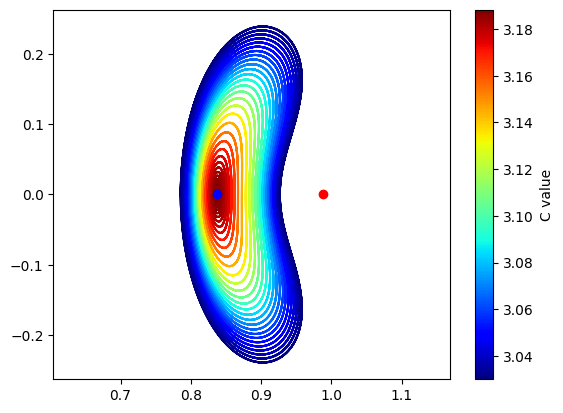
\includegraphics[width=0.49\textwidth]{images/L1.png}
    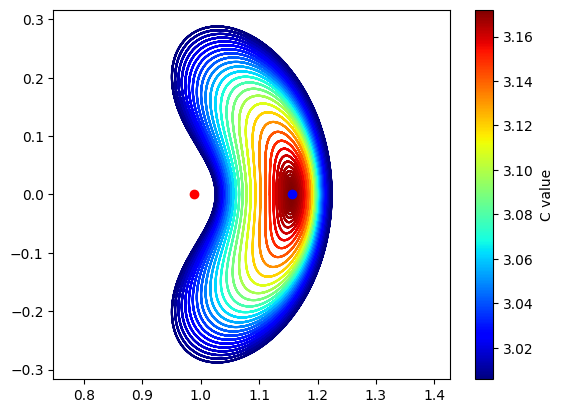
\includegraphics[width=0.49\textwidth]{images/L2.png}
    \caption{Lyapunov orbits around L1 and L2}
\end{figure}
\subsection*{Isoenergetic Lyapunov orbits}
As per request, two pair of isoenergetic Lyapunov orbits is seeked. Two orbits in the Jacobi range
$C_J = [3.1370, 3.1493]$ are found in the family around L1 from the previously computed family. 
A bisection method on the solution step $ds$ is employed to find the two pairs. The following pseudocode illustrates the procedure:
\begin{verbatim}
    ds_a = 0
    ds_b = next_orb_ds
    while abs(C_J - C_J_target) > tol:
        ... # Compute nonlinear Lyapunov orbit with ds_guess
        if C_J > C_J_target:
            ds_a = ds_guess
        else:
            ds_b = ds_guess
        ds_guess = (ds_a + ds_b)/2
   
\end{verbatim}




\chapter{Methodology}
% Your methodology content here

\chapter{Results}
% Your results content here

\chapter{Conclusion}
% Your conclusion content here

\end{document}